\documentclass[8pt]{beamer}
\usepackage[utf8]{inputenc}
\usepackage{xcolor}
\usepackage{colortbl}
\usepackage{epsfig}
\usepackage{cancel}
\usepackage{ulem}
\usepackage{threeparttable} % Joao Pela: 
\usepackage{amsmath}
\usepackage{hyperref}
\usepackage{feynmp}         % For latex produced Feynman Diagrams

% Rule for feynmp diagrams to be considered graphics
\DeclareGraphicsRule{*}{mps}{*}{}

% New compile sequence for feynmp
\makeatletter
\def\endfmffile{%
  \fmfcmd{\p@rcent\space the end.^^J%
          end.^^J%
          endinput;}%
  \if@fmfio
    \immediate\closeout\@outfmf
  \fi
  \ifnum\pdfshellescape=\@ne
    \immediate\write18{mpost \thefmffile}%
  \fi}
\makeatother

\usetheme{Madrid}

\author[João Pela]{J. Pela}
\title[VBF Higgs @ LHC-CMS]{VBF Higgs Searches @ LHC-CMS}
\subtitle{PhD 3 Months Report}
\institute{Imperial College London}
\date{2012-02-22}

% The log drawn in the upper right corner.
\logo{
\includegraphics[height=0.115\paperheight]{img/Logo_CMSICL.png}}

\begin{document}
\setlength{\unitlength}{1mm}

\begin{frame}
  \titlepage
\end{frame}

\begin{frame}{Introduction and Motivation}

  The current knowledge on the field of particle physics is summarized in the Standard Model. Its success comes 
  from explaining a wide variety of experimental results.

  \begin{block}{But still it is incomplete:}

  \begin{itemize}  
    \item Does not include the physics of dark energy or a full theory of gravity (like general relativity).
    \item Does not contain a dark matter candidate.
    \item Needs the inclusion of a \uline{spontaneous symmetry breaking mechanism} to explain masses of the weak bosons:
    \begin{itemize}
      \item The easiest way: Higgs Mechanism
      \item Suggests: new particle the \uline{Higgs boson}
    \end{itemize}
  \end{itemize}

  \end{block}

  \begin{block}{After 2 years of operation the experiments at the LHC have:}

\begin{itemize}
  \item Narrowed down the allows mass range for the SM Higgs having excluded at 95\% confidence level the range 127-600 $GeV$. 
  \item Seen hits of a possible signal around 124 GeV (significance of 1.5$\sigma$ after LEE).
\end{itemize}

  \end{block}  

Predicted running condition for 2012 will provide enough data to discover of exclude a SM Higgs.

\end{frame}

\begin{frame}{SM Higgs Production Processes}

\begin{block}
  
\begin{table}
  
\begin{tabular}{cc}

\begin{fmffile}{feynmanDiagram_GFHiggs}
  \fmfframe(0,5)(0,5){
  \begin{fmfgraph*}(40,20)
    \fmfleft{g1,g2} \fmfright{H'}
    \fmf{gluon}{g1,t1}
    \fmf{gluon}{g2,t2}
    \fmf{fermion,tension=0,label=$t$,label.side=left}{t1,t2}
    \fmf{fermion,label=$t$,label.side=left}{t2,H}
    \fmf{fermion,label=$\bar{t}$}{H,t1}
    \fmf{boson}{H,H'}
    \fmflabel{$H^0$}{H'}
    \fmflabel{$g_1$}{g1}
    \fmflabel{$g_2$}{g2}
  \end{fmfgraph*}
  }
\end{fmffile}

(1) &

\begin{fmffile}{feynmanDiagram_VBFHiggs}
  \fmfframe(0,5)(0,5){
  \begin{fmfgraph*}(40,20)
    \fmfleft{P1,P2} \fmfright{P1',H',P2'}
    \fmf{fermion}{P1,g1}
    \fmf{fermion}{P2,g2}
    \fmf{boson,label=$W/Z^0$,label.side=left}{g1,H}
    \fmf{boson,label=$W/Z^0$,label.side=left}{H,g2}
    \fmfdot{H,g1,g1}
    \fmf{boson,tension=0.2}{H,H'}
    \fmf{fermion}{g1,P1'}
    \fmf{fermion}{g2,P2'}
    \fmflabel{$H^0$}{H'}
    \fmflabel{$q_1$}{P1}
    \fmflabel{$q_2$}{P2}
    \fmflabel{$q_1'$}{P1'}
    \fmflabel{$q_2'$}{P2'}
  \end{fmfgraph*}
  }
\end{fmffile}
(2) \\
\begin{fmffile}{feynmanDiagram_ttFHiggs}
  \fmfframe(0,5)(0,5){
  \begin{fmfgraph*}(40,20)
    \fmfleft{g2,g1} 
    \fmfright{t2',H',t1'}
    \fmf{gluon}{g2,t2}
    \fmf{gluon}{g1,t1}
    \fmf{fermion}{t2',t2}
    \fmf{fermion,label.side=right,label=$t$}{t2,H}
    \fmf{fermion,label.side=right,label=$\bar{t}$}{H,t1}
    \fmf{fermion}{t1,t1'}
    \fmf{boson,tension=0.5}{H,H'}
    \fmflabel{$H^0$}{H'}
    \fmflabel{$g_1$}{g1}
    \fmflabel{$g_2$}{g2}
    \fmflabel{$t$}{t1'}
    \fmflabel{$\bar{t}$}{t2'}
  \end{fmfgraph*}
  }
\end{fmffile}
(3) &

\begin{fmffile}{feynmanDiagram_WZstrahlung}
  \fmfframe(0,5)(0,5){
  \begin{fmfgraph*}(40,20)
    \fmfleft{q2,q1} \fmfright{H',V'}
    \fmf{fermion}{v1,q2}
    \fmf{fermion}{q1,v1}
    \fmf{boson,label=$W/Z$}{v1,v2}
    \fmf{boson}{v2,V'}
    \fmf{boson}{v2,H'}
    \fmflabel{$H^0$}{H'}
    \fmflabel{$W/Z$}{V'}
    \fmflabel{$q$}{q1}
    \fmflabel{$\bar{q}$}{q2}
  \end{fmfgraph*}
  }
\end{fmffile}
(4)

\end{tabular}
\caption{SM Higgs production ordered by highest cross section at the LHC. (1) Gluon Fusion, (2) Vector Boson Fusion, (3) $t\bar{t}$ Fusion and (4) $W/Z$ associated production.}
\end{table}

\end{block}

\end{frame}

\begin{frame}{Higgs Production Cross Section\& Branching Ratio}

\begin{columns}
  
  \column[t]{5.75cm}
  \begin{block}{SM Higgs Cross Section}
    
    \begin{center}
      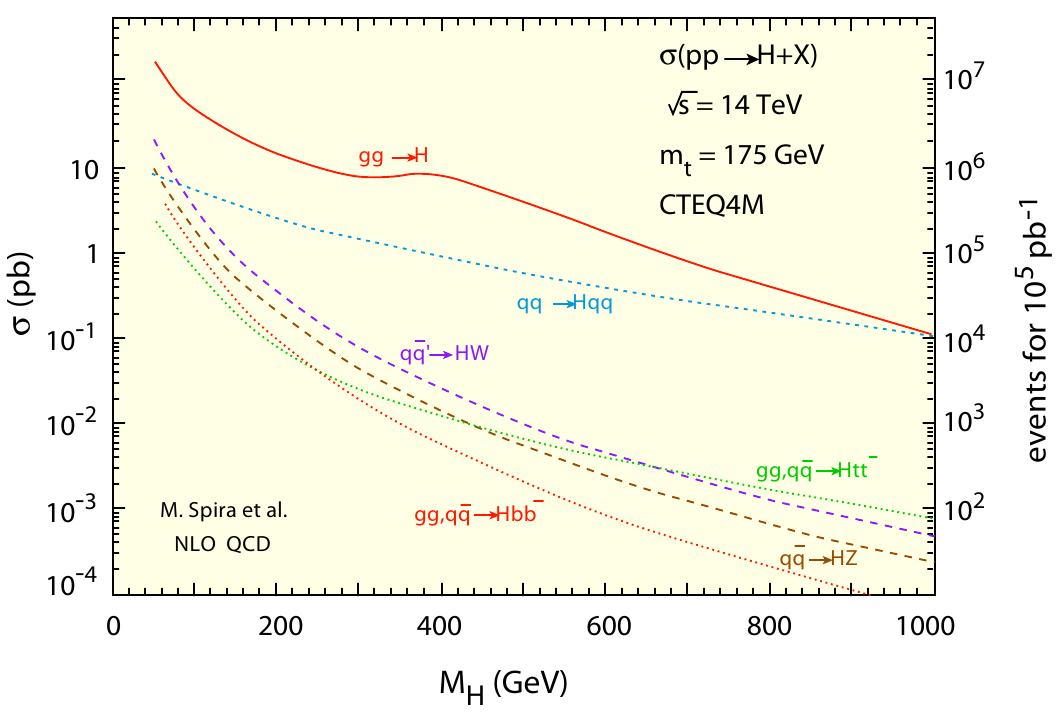
\includegraphics[width=1.00\textwidth]{img/SMHiggs_XSec.png} 
    \end{center}

  \end{block}

  \column[t]{5.75cm}
  \begin{block}{Branching Ratio}

    \begin{center}
      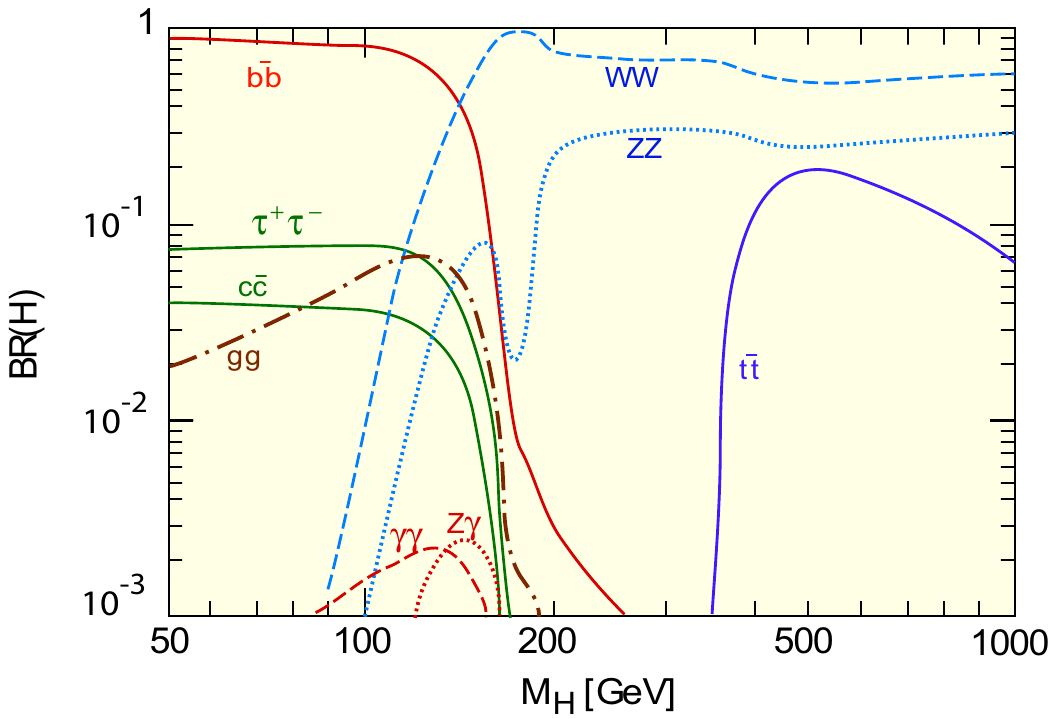
\includegraphics[width=1.00\textwidth]{img/SMHiggs_BR.png} 
    \end{center}
    
  \end{block}

\end{columns}

  \begin{block}

For the currently allowed experimental mass range for the SM Higgs:
\begin{itemize}
  \item VBF Signature is a factor of $\sim10$ lower then gluon fusion.
  \item Most important/possible decays $b\bar{b}$, $\tau\bar{\tau}$, $c\bar{c}$, $gg$, $\gamma\gamma$ and $Z\gamma$. 
\end{itemize}

  \end{block}

\end{frame}

\begin{frame}{Why VBF Higgs?}

\begin{block}{Theoretical}

  \begin{itemize}
    \item Observe Higgs on this channel and measure its cross section and branching ratios for each decay.
    \item Measure Higgs coupling with Weak Bosons and fermions.
    \begin{itemize}
      \item Higgs properties.
      \item Differentiate between SM Higgs and BSM Higgs.
    \end{itemize}
    \item Primary channel for discovery if Higgs only decays invisibly.
  \end{itemize}

\end{block} 

\begin{block}{Experimental}

  VBF cross section is one order of magnitude lower than gluon fusion, but: 
  \begin{itemize}
    \item Two additional Forward Jets (can be used for tagging).
    \item Low hadronic activity in central region (no colour exchange between quarks).
    \item Higgs decay products (channel dependent) are isolated in central area, allowing easier properties studies.
  \end{itemize}

\end{block} 

\end{frame}

\begin{frame}{The LHC-CMS Experiment}
 
  \begin{block}{Large Hadron Collider}

    \begin{columns}

      \column[t]{5.5cm}
      \begin{center}
        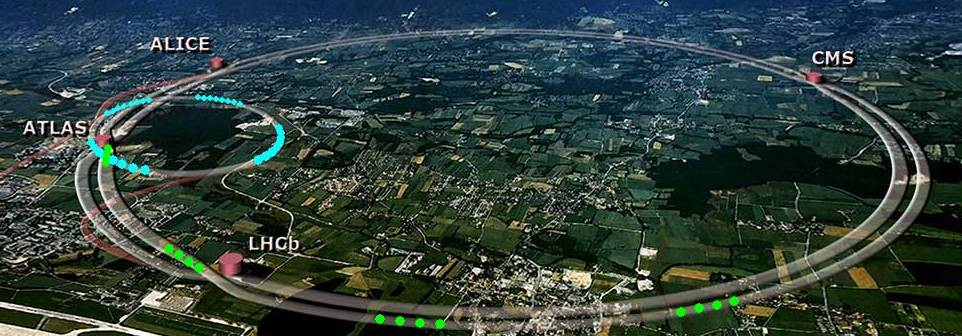
\includegraphics[width=1.00\textwidth]{img/LHCMap.jpg} 
      \end{center}

      \column[t]{5.5cm}

      \begin{itemize}
        \item Located at Franco-Swiss border near Geneva, Switzerland.
        \item Synchrotron Machine (currently the most powerful in activity).
        \item Can collide protons up to $\sqrt{s}=14$ $TeV$ (during 2012 $\sqrt{s}=8$ $TeV$).
      \end{itemize}

    \end{columns}

  \end{block}

  \begin{block}{Compact Muon Solenoid}

    \begin{columns}
      \column[t]{6.5cm}

      \begin{itemize}
        \item Located at LHC Point 5.
        \item General purpose experiment.
        \item Objective of studying a broad spectrum of physics.
        \item Classical onion structure.
        \item Most powerful solenoid ever built (3.8 $T$).
      \end{itemize}  

      \column[t]{4.5cm}
      \begin{center}
        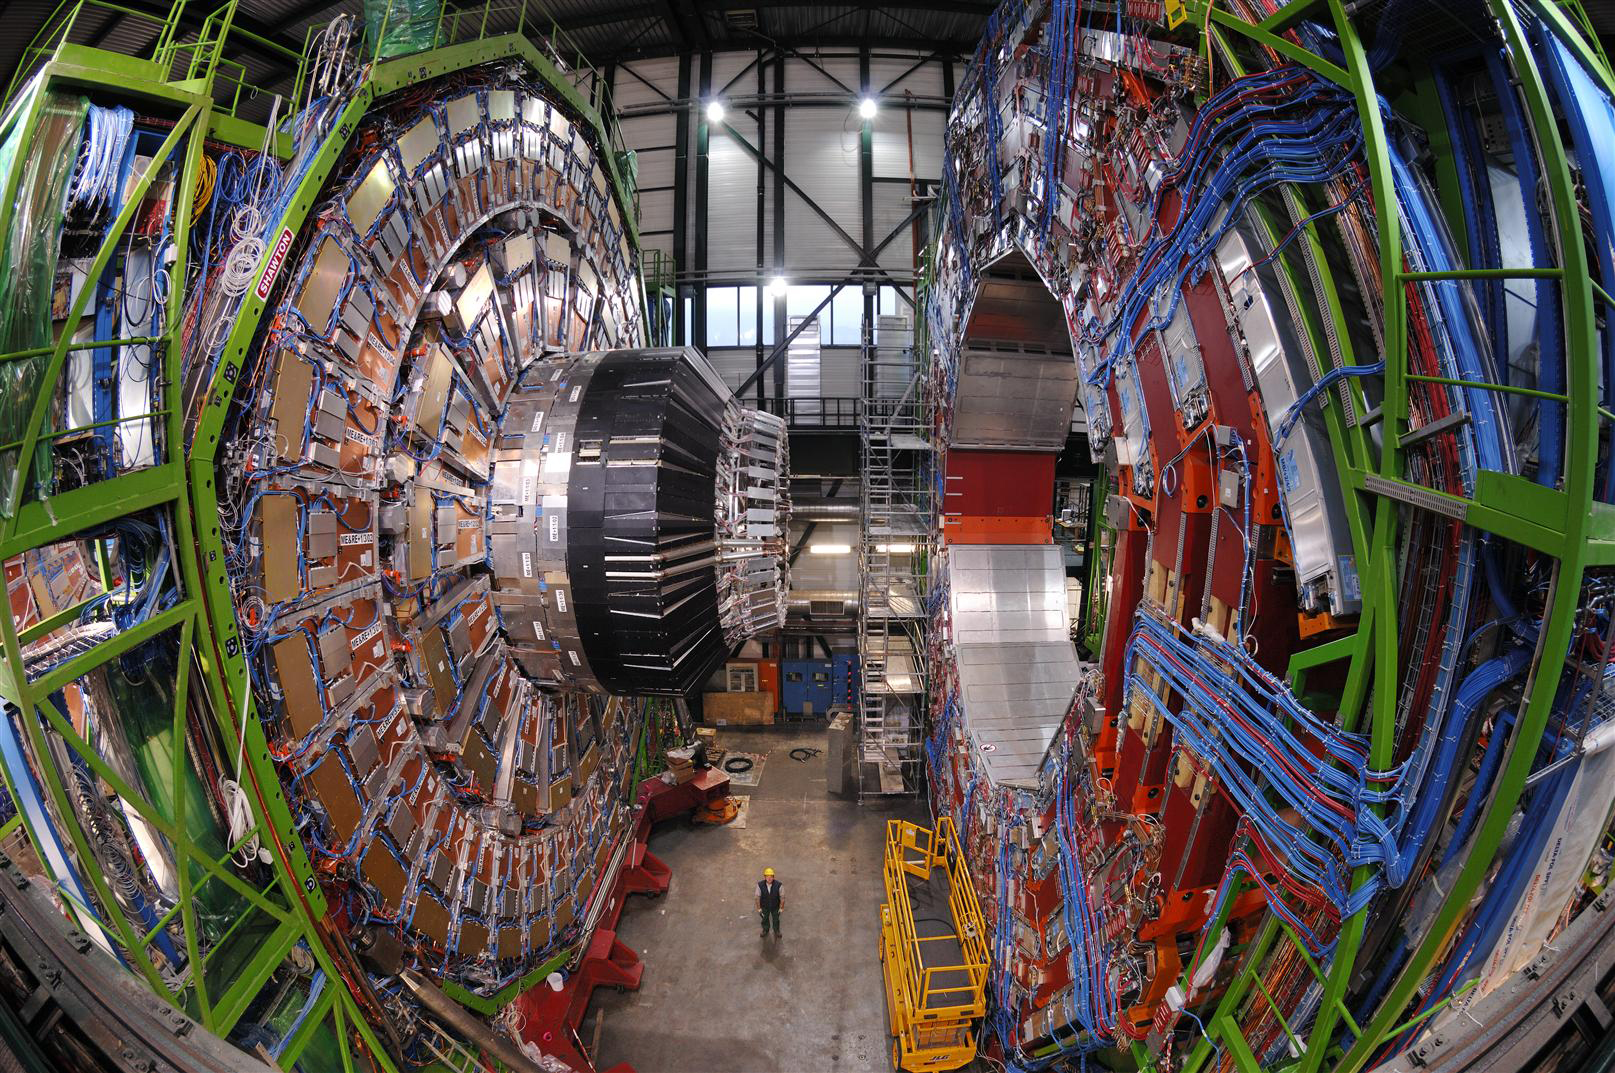
\includegraphics[width=1.00\textwidth]{img/CMSOpen.jpg} 
      \end{center}

    \end{columns}

  \end{block}

\end{frame}

\begin{frame}{VBF Signature @ CMS}

  \begin{columns}

    \column[t]{5.0cm}
    \begin{block}{VBF $H^0 \rightarrow \tau \tau$ simulated event}

      \begin{center}
        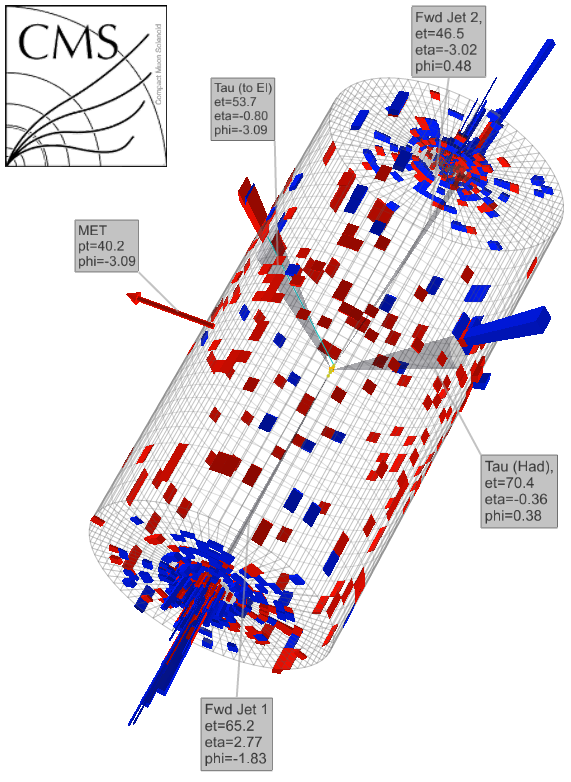
\includegraphics[width=1.00\textwidth]{img/EventDisplay_VBF_HToTauTau_El-Had.png} 
      \end{center}

    \end{block}

    \column[t]{6.5cm}
    \begin{block}{Topology}
      
      \begin{itemize}
        \item Two forward jet with resonable $p_T$
        \begin{itemize}
          \item High $\Delta\eta$ and low $\Delta\phi$.
          \item Low hadronic activity between jets (no color exchange between quarks).
          \item High dijet invariant mass.
          \item Higgs decay products on oposite direction of the dijet (signature specif)
        \end{itemize}
        \item Additional Higgs Decay products signature.
      \end{itemize}

    \end{block}

    \begin{block}{Objects $\eta$ distribution}
      
      \begin{center}
        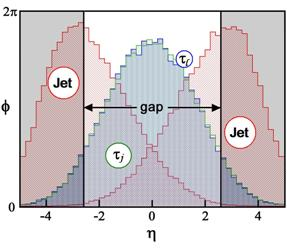
\includegraphics[width=0.60\textwidth]{img/ObjectsRapidityGap.jpeg} 
      \end{center}

    \end{block}

  \end{columns}

\end{frame}

\begin{frame}{Work and Plans}
  
  \begin{block}{Current and finished work}

    \begin{itemize}
      \item L1 Rates Study for the VBF Higgs to invisible study (finished, to be revisited)
      \item Development of dedicated Inclusive L1 Trigger (ongoing)
    \end{itemize}

  \end{block}

  \begin{block}{Plans}

    \begin{itemize}
      \item Participate on the L1-HLT Inclusive VBF Trigger development, commissioning and maintenance.   
      \item Develop a data analysis based on a VBF Higgs Channel aimed at observation and properties measurement.
      \item Participate on the trigger related effort (DQM, upgrades,...).
    \end{itemize}
    
  \end{block}

\end{frame}

\begin{frame}{Rate Studies for a Higgs to Invisible L1 Trigger}

  Final resulst for this L1 rates study. Always requiring a dijet with $\Delta\eta>3$ and testing 
  each variable on 4 $\Delta\phi$ points (no cut, $<2.5$, $<2.1$ and $<1.8$).

\begin{block}{$5e33$ - $<PU>=28$}

  \begin{columns}

  \column[t]{5.5cm}  
\begin{footnotesize} 
\begin{tabular}{|c||c|c|c|c|}
\hline
\multicolumn{5}{|c|}{MET [GeV] (with Dijet $E_\bot>20$ [GeV])} \\
\hline
$\Delta\phi$ & no cut & 2.5 & 2.1 & 1.8 \\
\hline
10kHz        &     32 &  32 &  32 &  32 \\
5kHz         &     35 &  35 &  35 &  35 \\
\cellcolor{green}2kHz &\cellcolor{green}      41 &  41 &  41 &  41 \\
1kHz         &     47 &  47 &  47 &  46 \\
500Hz        &     54 &  54 &  54 &  53 \\
\hline
\end{tabular}
\end{footnotesize}

  \column[t]{5.5cm}  
\begin{footnotesize} 
\begin{tabular}{|c||c|c|c|c|}
\hline
\multicolumn{5}{|c|}{Dijet $E_\bot$ [GeV] (with $MET>30$ [GeV])} \\
\hline
$\Delta\phi$ & no cut & 2.5 & 2.1 & 1.8 \\
\hline
10kHz        &     28 &  28 &  24 &  24 \\
5kHz         &     32 &  32 &  32 &  32 \\
\cellcolor{green} 2kHz         &\cellcolor{green}      52 &  48 &  44 &  44 \\
1kHz         &     68 &  68 &  64 &  64 \\
500Hz        &     92 &  92 &  88 &  88 \\
\hline
\end{tabular}
\end{footnotesize}

  \end{columns}

\end{block}

Results used to define the working point for this trigger, which was already proposed to the TSG to be included
on a future L1 Trigger menus. Proposed trigger:
\begin{itemize}
  \item Dijet $E_\bot>20$ GeV + fwd/bkwd + $\Delta\eta_{jj}>3$ + $MET>40$ GeV
  \item Dijet $E_\bot>50$ GeV + fwd/bkwd + $\Delta\eta_{jj}>3$ + $MET>30$ GeV
\end{itemize}


\begin{block}{$7e33$ - $<PU>=32$}

  \begin{columns}

  \column[t]{5.5cm}  
\begin{footnotesize} 
\begin{tabular}{|c||c|c|c|c|}
\hline
\multicolumn{5}{|c|}{MET [GeV] (with Dijet $p_\bot>20$ [GeV])} \\
\hline
$\Delta\phi$ & no cut & 2.5 & 2.1 & 1.8 \\
\hline
10kHz        &     36 &  36 &  36 &  36 \\
5kHz         &     40 &  40 &  40 &  40 \\
2kHz         &     47 &  47 &  47 &  46 \\
1kHz         &     54 &  54 &  54 &  54 \\
500Hz        &     67 &  66 &  66 &  64 \\
\hline
\end{tabular}
\end{footnotesize}

  \column[t]{5.5cm} 
\begin{footnotesize}  
\begin{tabular}{|c||c|c|c|c|}
\hline
\multicolumn{5}{|c|}{Dijet $p_\bot$ [GeV] (with $MET>30$ [GeV])} \\
\hline
$\Delta\phi$ & no cut & 2.5 & 2.1 & 1.8 \\
\hline
10kHz        &     32 &  32 &  32 &  32 \\
5kHz         &     40 &  40 &  40 &  40 \\
2kHz         &     64 &  60 &  60 &  56 \\
1kHz         &     76 &  76 &  76 &  76 \\
500Hz        &    100 & 100 &  96 &  92 \\
\hline
\end{tabular}
\end{footnotesize}

  \end{columns}

\end{block}

\end{frame}

\begin{frame}{Development of dedicated Inclusive L1 Trigger}

It would be desirable to have a dedicated Inclusive L1 Trigger (i.e. Higgs decay independent):
\begin{block}

\begin{itemize}
  \item Single trigger for all VBF signature analysis
  \begin{itemize}
    \item Less systematics comparing analysis
    \item More people using a trigger usually means it will become better understood
  \end{itemize}
  \item No dependence in the Higgs decay
  \begin{itemize}
    \item Get all possible decays (thus a Model Independent trigger)
  \end{itemize}
  \item Can be used for a WW scattering analysis. 
\end{itemize}

\end{block}

Trigger would be based only on the forward dijet present on the VBF signature
\begin{block}{Types of trigger studied}
  
  Always requiring a dijet with $\Delta\eta>3$ and testing each variable on 4 $\Delta\phi$ points (no cut, $<2.5$,
  $<2.1$ and $<1.8$).

  \begin{itemize}
    \item Invariant Mass
    \begin{itemize}
      \item Benefit from the very high $M_{inv}$ of the dijet system.
      \item Not yet implemented on the L1 Hardware but possible.
    \end{itemize}
    \item Transverse Invariant Mass
    \begin{itemize}
      \item Better suppression of QCD, less PU dependency and lower error associated (only x-y dependence).
      \item Not yet implemented on the L1 Hardware but possible.
    \end{itemize}
    \item HT (Vectorial Sum of the Hadronic Energy) 
    \begin{itemize}
      \item Theoretically best variable to separate signal from background.
      \item \uline{Already implemented} on L1 Hardware.
    \end{itemize}
  \end{itemize}

\end{block}

\end{frame}

\begin{frame}{Results}

\begin{block}{Trigger types:}
  
  \begin{itemize}
    \item $M_{Inv}$: Unusable. To get acceptable rates have to cut too high on Jet $p_\bot$ or $M_{Inv}$ 
                     losing signal efficiency.
    \item $M_{\bot}$: Promising. Rate of 5kHz with $MT>50GeV$ no $\Delta\phi$ cut and dijet $p_\bot \sim 45GeV$
                      giving a signal efficiency of $\lesssim70\%$ (see R. Lane talk) 
    \item $HT$: Most promising. Rate of 5kHz with $HT>100GeV$ no $\Delta\phi$ cut and dijet $p_\bot \sim 40GeV$ giving 
                a signal efficiency of $\lesssim98\%$ (see R. Lane talk) 
  \end{itemize}

\end{block}

\begin{columns}

  \column[t]{5.0cm}
  \begin{block}{Rate(dijet $p_\bot$) for $HT>100GeV$}
    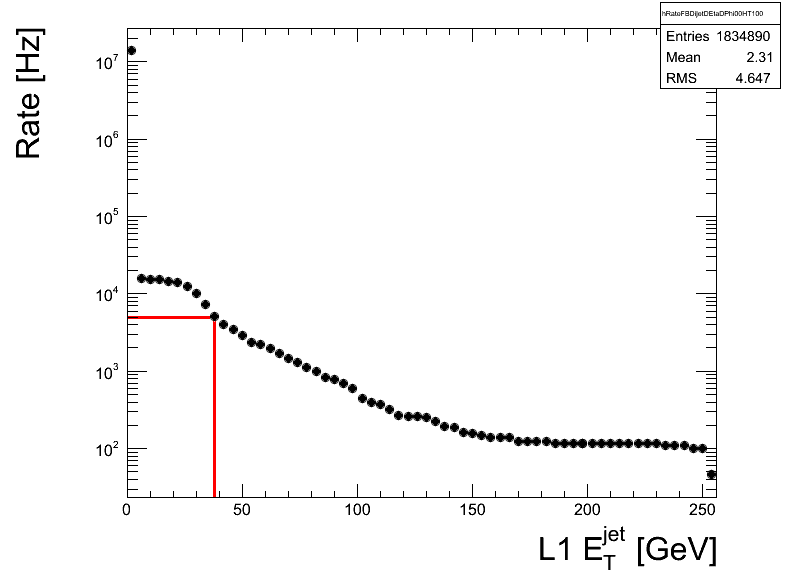
\includegraphics[width=1.00\textwidth]{img/PU28_5e33_RateFBDijetDEtaDPhi00HT100.png} 
  \end{block}

  \column[t]{5.5cm}
  \begin{block}{HT efficiency}
    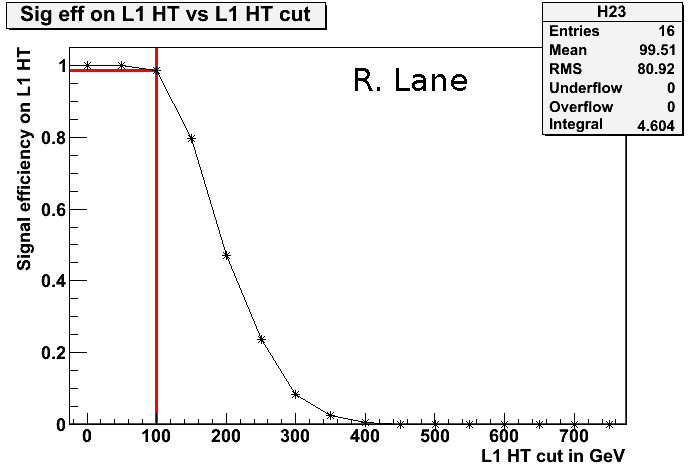
\includegraphics[width=1.00\textwidth]{img/sig_eff_l1_ht.png} 
  \end{block}

\end{columns}

\end{frame}

\begin{frame}{Conclusions}
 
  \begin{block}{Overview}

    \begin{itemize}
      \item There will be a VBF Higgs to Invisible dedicated trigger for 2012. 
      \item Most likely an inclusive VBF trigger will be included soon, which should cover most of the 2012 data.
      \item 2012 will be an exciting year for all the LHC experiments. 
      \item Imperial College CMS Group highly involved on the trigger effort for VBF analysis.
      \begin{itemize}
        \item Which will evolve quickly with data to a full analysis effort aimed at publication of the
              (soon to be discovered) Higgs Boson properties.
      \end{itemize}
    \end{itemize}

  \end{block}
   
\end{frame}

\end{document}